% Provenance (never printed): old premiere S material on the formation of fossil
% fuels (preserved organic matter, burial, oil window, migration, trap, coal).
% Burial history of the invented Merrow Basin from figdata/grade-11/oil_window.py
% (constant geotherm, no compaction). Rifts and passive margins after the USGS
% West-Central Coastal Province fact sheet (2023-3028). Folds are defined in
% g12.02 mountain-building (Sync 0): the anticline is told in prose here, never
% defined. Sedimentary basins compared, diagenesis: Year 1/2.
\chapter{Geologi Batu Bara, Minyak Bumi, dan Gas}\label{ch:g11:fossil-fuel-geology}

Sebongkah serpih hitam yang diambil dari sebuah tambang \omterm{def:g11:fossil-fuel-geology:coal}{batu bara} tua di
Pennsylvania memuat daun-daun tumbuhan mirip pakis, pipih dan keperakan di atas
batuan yang gelap. Tumbuhan itu tumbuh di sebuah rawa lebih dari tiga ratus
juta tahun yang lalu, pada zaman Karbon; karena terkubur sebelum sempat membusuk,
daun-daun itu mempertahankan bentuknya, dan karbon tumbuh-tumbuhan rawa itu
menjadi \omterm{def:g11:fossil-fuel-geology:coal}{batu bara}. Minyak bumi dan gas, yang kini dipompa dari anjungan di
tengah laut, asal-usulnya sejenis: sisa-sisa makhluk hidup yang luput dari
pembusukan, lalu terkubur dan terpanaskan. Bab ini mengikuti karbon yang
terkubur itu dari rawa dan dasar laut sampai ke lapisan \omterm{def:g11:fossil-fuel-geology:coal}{batu bara} dan ladang
minyak.
% ledger: photo:g11-fossil-plants, ics:base.Carboniferous, ics:base.Permian, earle:coal-formation, earle:organic-preservation

\begin{omfigure}
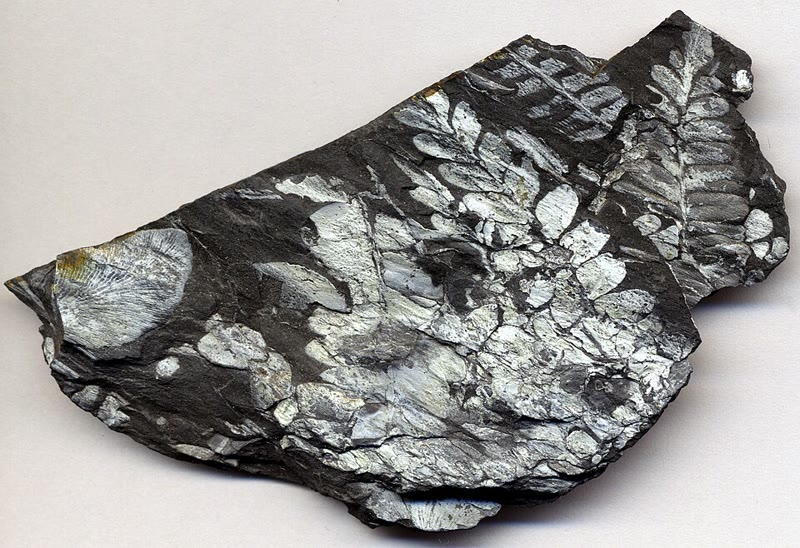
\includegraphics[height=4.4cm]{images/book2/g11-stjohn-fossil-plants.jpg}\hspace{0.03\linewidth}%
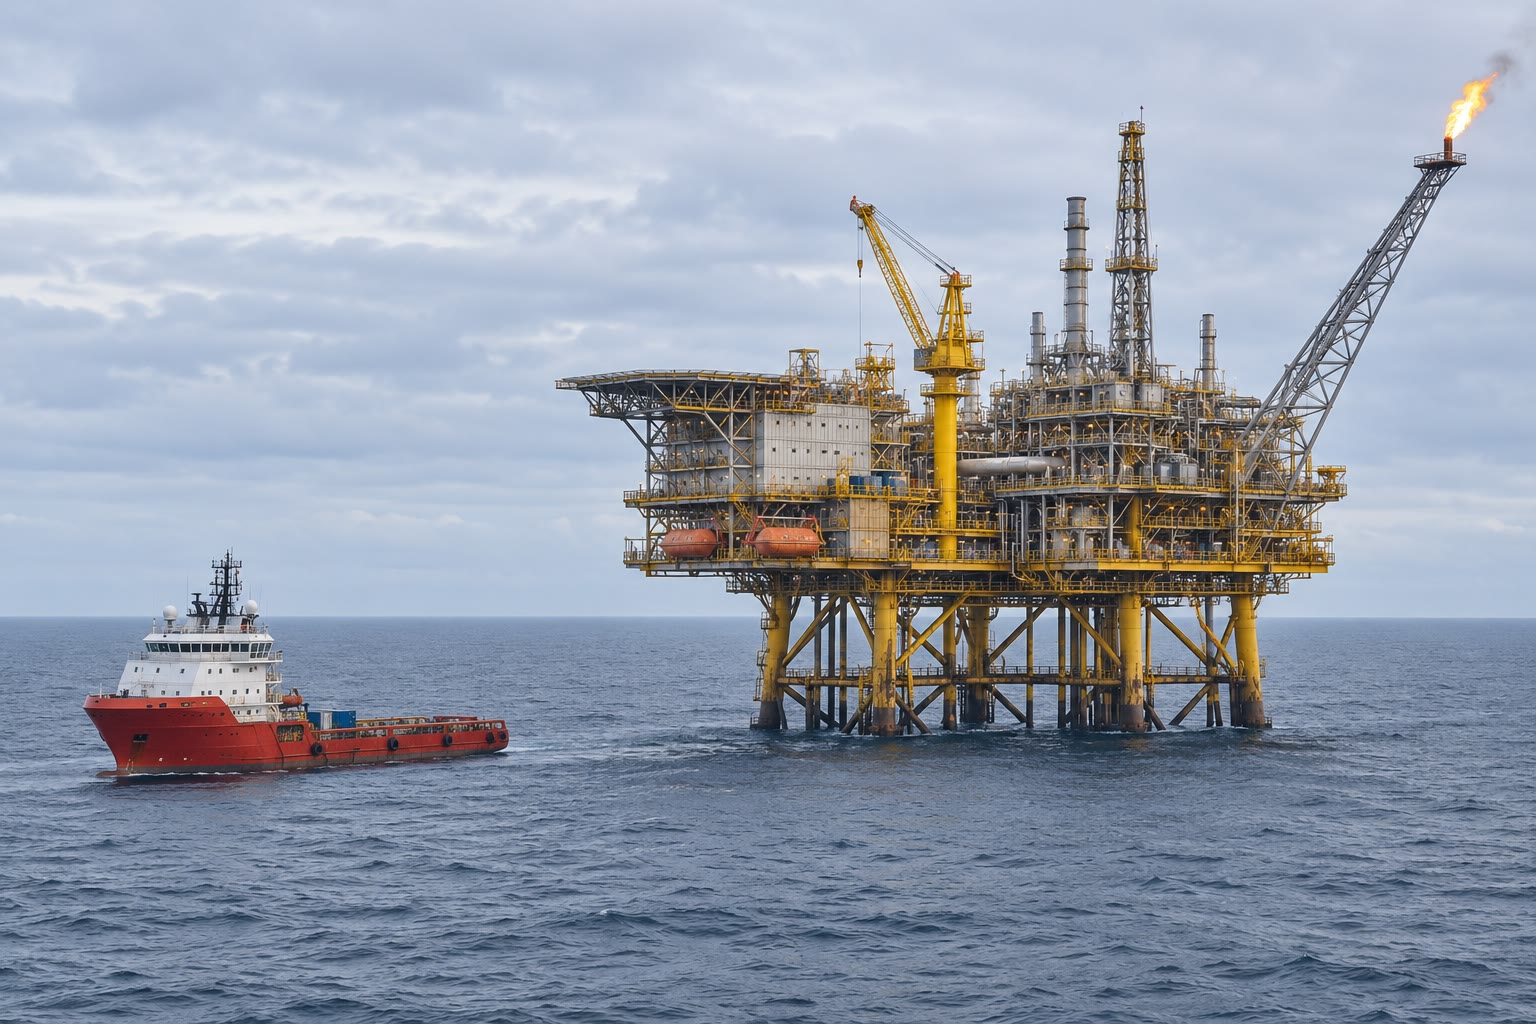
\includegraphics[height=4.4cm]{images/book2/ai/g11-offshore-platform.jpg}

{\small Kiri: daun tumbuhan fosil dalam serpih yang kaya karbon dari sebuah
tambang \omterm{def:g11:fossil-fuel-geology:coal}{batu bara} tua, Pennsylvania, zaman Karbon; lebar bongkahnya sekitar
\qty{10}{cm}. Foto James St.~John (CC~BY~2.0). Kanan: anjungan produksi minyak
dan gas di laut (ilustrasi AI).}
\end{omfigure}
% ledger: photo:g11-fossil-plants

\begin{recall}
\omterm{def:g11:fossil-fuel-geology:coal}{Batu bara}, minyak bumi, dan gas alam adalah bahan bakar fosil: minyak bumi dan
gas adalah campuran hidrokarbon, yaitu senyawa karbon dan hidrogen, dan
pembakaran bahan bakar fosil melepaskan energi dan karbon dioksida (buku-buku
kimia). Tumbuhan dan alga membuat bahan organik dari karbon dioksida dan air
melalui fotosintesis (buku-buku biologi). \omterm{def:g11:fossil-fuel-geology:coal}{Batu bara}, minyak bumi, dan gas
berasal dari bahan organik yang terkubur dalam sedimen, dan tersimpan dalam
batuan sedimen (Buku 1, kelas 9). Batuan bersifat berpori bila mempunyai
ruang-ruang kosong, dan permeabel bila air dapat mengalir melaluinya (Buku 1,
kelas 6). Suhu naik dengan kedalaman di sepanjang \omterm{def:g11:lithosphere-asthenosphere:geotherm}{geoterm}, sebesar 25 sampai
\qty{30}{\degreeCelsius} per kilometer pada beberapa kilometer pertama
(\cref{ch:g11:lithosphere-asthenosphere}).
\end{recall}
% ledger: usgs:gradient-29, earle:organic-preservation

\section{Mengawetkan bahan organik}

Sebagian besar bahan organik tidak pernah menjadi bahan bakar. Sehelai daun
mati atau sebutir alga mati dimakan oleh hewan dan bakteri atau bereaksi dengan
oksigen udara: dalam beberapa minggu atau beberapa tahun karbonnya telah
kembali ke atmosfer sebagai karbon dioksida. Bahan organik hanya bertahan di
tempat yang terputus dari oksigen --- di dasar rawa yang airnya tergenang, atau
di dasar laut atau dasar danau yang airnya tidak mengandung oksigen. Bila
terkubur di sana di bawah sedimen lain, bahan itu dapat tersimpan selama
puluhan atau ratusan juta tahun.
% ledger: earle:organic-preservation

\omterm{def:g11:fossil-fuel-geology:coal}{Batu bara} sebagian besar berasal dari tumbuhan darat yang menumpuk di rawa.
Minyak bumi dan gas sebagian besar berasal dari alga mikroskopis dan plankton
lain di laut: di tempat perairan permukaannya sangat produktif, plankton mati
turun seperti hujan ke dasar laut cukup cepat sehingga sebagiannya luput dari
pembusukan, lalu terkubur di dalam lumpur.
% ledger: earle:coal-formation, earle:oil-window

\begin{definition}[Batuan sumber; kerogen]\label{def:g11:fossil-fuel-geology:source-rock}
Yang disebut \emph{kerogen}\index{kerogen} adalah bahan organik yang tersebar
dalam batuan sedimen, berupa partikel-partikel kecil yang tidak larut dalam
pelarut organik. Yang disebut \emph{batuan sumber}\index{batuan sumber} adalah
batuan sedimen yang kaya kerogen, tempat minyak bumi dan gas terbentuk ketika
batuan itu terkubur dan terpanaskan.
\end{definition}
% ledger: peters08:kerogen, earle:migration-traps

Sebagian besar \omterm{def:g11:fossil-fuel-geology:source-rock}{batuan sumber} berupa serpih dan batu lumpur, yang diendapkan
sebagai lumpur yang kaya bahan organik. Di dekat permukaan, \omterm{def:g11:fossil-fuel-geology:source-rock}{kerogennya} tetap
padat: bakteri yang hidup tanpa oksigen mengubah sebagian bahan organik itu
menjadi metana, tetapi sebagian besar metana itu lolos kembali ke permukaan.
Pembentukan minyak bumi memerlukan kalor, dan kalor memerlukan kedalaman.
% ledger: earle:oil-window, peters08:kerogen

\section{Penimbunan dan pematangan}

\begin{definition}[Cekungan sedimen]\label{def:g11:fossil-fuel-geology:basin}
Yang disebut \emph{cekungan sedimen}\index{cekungan sedimen} adalah wilayah
kerak yang turun selama jutaan tahun, sehingga sedimen menumpuk di dalamnya,
sering kali sampai setebal beberapa kilometer.
\end{definition}
% ledger: usgs23:rift-salt

Dalam cekungan yang sedang turun, setiap lapisan terkubur makin lama makin
dalam di bawah lapisan-lapisan yang menumpuk di atasnya. Selagi turun, lapisan
itu mengikuti \omterm{def:g11:lithosphere-asthenosphere:geotherm}{geoterm}: lapisan itu terpanaskan. \omterm{def:g11:fossil-fuel-geology:source-rock}{Kerogennya} perlahan-lahan
dimasak, molekul-molekulnya yang besar dipecah menjadi molekul-molekul
minyak bumi dan gas yang lebih kecil.
% ledger: earle:oil-window

\begin{definition}[Pematangan; jendela minyak; jendela gas]\label{def:g11:fossil-fuel-geology:oil-window}
Yang disebut \emph{pematangan}\index{pematangan} \omterm{def:g11:fossil-fuel-geology:source-rock}{batuan sumber} adalah perubahan
\omterm{def:g11:fossil-fuel-geology:source-rock}{kerogennya} menjadi minyak bumi dan gas ketika batuan itu terkubur dan
terpanaskan. Yang disebut \emph{jendela minyak}\index{jendela minyak} adalah
selang suhu, dari sekitar 60 sampai \qty{120}{\degreeCelsius}, tempat \omterm{def:g11:fossil-fuel-geology:source-rock}{kerogen}
terutama membentuk minyak bumi. Di atas sekitar \qty{120}{\degreeCelsius},
dalam \emph{jendela gas}\index{jendela gas}, \omterm{def:g11:fossil-fuel-geology:source-rock}{kerogen} terutama membentuk metana.
\end{definition}
% ledger: earle:oil-window, magoon00:tps

Karena suhu naik dengan kedalaman, \omterm{def:g11:fossil-fuel-geology:oil-window}{jendela minyak} juga merupakan sebuah selang
kedalaman. Di tempat \omterm{def:g11:lithosphere-asthenosphere:geotherm}{geotermnya} berupa garis lurus, selang itu mudah dicari.

\begin{proposition}[Kedalaman jendela minyak]\label{prop:g11:fossil-fuel-geology:window-depth}
Misalkan suhu di permukaan adalah $T_0$ dan naik dengan kedalaman $z$ menurut
\omterm{def:g11:lithosphere-asthenosphere:geotherm}{gradien geotermal} $G$ yang tetap: $T = T_0 + G z$. Maka \omterm{def:g11:fossil-fuel-geology:oil-window}{jendela minyak} terletak
di antara kedalaman
\[
  z_{\text{atas}} = \frac{60 - T_0}{G}
  \qquad\text{dan}\qquad
  z_{\text{bawah}} = \frac{120 - T_0}{G},
\]
dengan suhu dalam \unit{\degreeCelsius}. Tebalnya $60/G$: makin curam \omterm{def:g11:lithosphere-asthenosphere:geotherm}{geotermnya},
makin dangkal dan makin tipis jendelanya.
\end{proposition}
% ledger: earle:oil-window

\begin{proof}
Puncak jendela adalah kedalaman tempat $T_0 + G z = 60$, yaitu
$z = (60 - T_0)/G$; dasarnya adalah tempat $T_0 + G z = 120$. Selisihnya
$(120 - 60)/G = 60/G$.
\end{proof}

Dengan permukaan bersuhu \qty{20}{\degreeCelsius} dan gradien
\qty{30}{\degreeCelsius} per kilometer, \omterm{def:g11:fossil-fuel-geology:oil-window}{jendela minyak} terletak antara
$40/30 \approx \qty{1.3}{km}$ dan $100/30 \approx \qty{3.3}{km}$. Pada lubang
bor di seluruh Amerika Serikat, gradien itu rata-rata
\qty{29}{\degreeCelsius} per kilometer, \num{25} di timur dan \num{34}
di barat; \omterm{def:g11:fossil-fuel-geology:source-rock}{batuan sumber} biasanya harus terkubur lebih dari sekitar
\qty{2}{km} sebelum menghasilkan minyak bumi. Bila tidak ada pengukuran
\omterm{def:g11:fossil-fuel-geology:source-rock}{kerogen}, ahli geologi minyak bumi menganggap \omterm{def:g11:fossil-fuel-geology:source-rock}{batuan sumber} yang terkubur di bawah
lebih dari sekitar \qty{3}{km} batuan yang lebih muda sebagai batuan yang telah
matang.
% values (oil_window.py): z_top_km 1.3333, z_base_km 3.3333
% ledger: usgs:gradient-29, earle:oil-window, magoon00:tps

\begin{omfigure}
\begin{tikzpicture}
\begin{axis}[omrecord, omage, omdepth, name=burial, width=0.54\linewidth, height=5.6cm,
  xmin=0, xmax=170, ymin=0, ymax=4.5, xlabel={umur (juta tahun yang lalu)},
  ylabel={kedalaman (\unit{km})}, unbounded coords=jump, clip=false,
  xtick={0,20,...,160}, ytick={0,1,...,4}]
\fill[omProp!18] (axis cs:170,1.3333) rectangle (axis cs:0,3.3333);
\fill[omThm!12] (axis cs:170,3.3333) rectangle (axis cs:0,4.5);
\node[font=\scriptsize, anchor=west, text=omProp!80!black] at (axis cs:168,1.75) {jendela minyak};
\node[font=\scriptsize, anchor=west, text=omThm] at (axis cs:168,3.9) {jendela gas};
\node[font=\scriptsize, anchor=south west, text=black!60, inner sep=1pt] at (axis cs:168,1.3333) {\qty{60}{\degreeCelsius}};
\node[font=\scriptsize, anchor=south west, text=black!60, inner sep=1pt] at (axis cs:168,3.3333) {\qty{120}{\degreeCelsius}};
% computed in figdata/grade-11/oil_window.py (invented basin)
\addplot[black!45, line width=0.6pt] table[x=age, y=z150] {figdata/out/grade-11-oil_window-history.dat};
\addplot[black!45, line width=0.6pt] table[x=age, y=z120] {figdata/out/grade-11-oil_window-history.dat};
\addplot[black!45, line width=0.6pt] table[x=age, y=z95] {figdata/out/grade-11-oil_window-history.dat};
\addplot[black!45, line width=0.6pt] table[x=age, y=z66] {figdata/out/grade-11-oil_window-history.dat};
\addplot[black, line width=1.4pt] table[x=age, y=z165] {figdata/out/grade-11-oil_window-history.dat};
\draw[omDef, dashed, line width=0.8pt] (axis cs:80,0) -- (axis cs:80,4.5);
\node[font=\scriptsize, anchor=west, text=omDef, inner sep=1pt] at (axis cs:78,4.2) {antiklin terbentuk};
\fill[omThm] (axis cs:116.97,1.3333) circle (2pt);
\fill[omThm] (axis cs:51.24,3.3333) circle (2pt);
\node[font=\scriptsize, anchor=north east, inner sep=1pt] at (axis cs:100,2.3) {batuan sumber};
\end{axis}
\begin{axis}[omrecord, omdepth, at={(burial.east)}, anchor=west, xshift=1.7cm, width=0.34\linewidth, height=5.6cm,
  xmin=15, xmax=50, ymin=0, ymax=7, xlabel={gradien (\unit{\degreeCelsius/km})},
  ylabel={kedalaman (\unit{km})}]
% computed in figdata/grade-11/oil_window.py (proposition, surface at 20 degC)
\addplot[name path=top, omProp, line width=1pt] table[x=G, y=z_top] {figdata/out/grade-11-oil_window-windows.dat};
\addplot[name path=base, omThm, line width=1pt] table[x=G, y=z_base] {figdata/out/grade-11-oil_window-windows.dat};
\addplot[omProp!18] fill between[of=top and base];
\node[font=\scriptsize] at (axis cs:40,1.75) {jendela minyak};
\node[font=\scriptsize, anchor=south, text=omProp!80!black] at (axis cs:42,0.95) {puncak};
\node[font=\scriptsize, anchor=north west, text=omThm] at (axis cs:24,4.6) {dasar};
\end{axis}
\end{tikzpicture}

{\small Kiri: sejarah penimbunan Cekungan Merrow, sebuah cekungan rekaan (model
yang dihitung, pemadatan diabaikan). Setiap garis mengikuti satu lapisan
sepanjang waktu, sejak hari lapisan itu diendapkan di permukaan; garis yang
tebal adalah \omterm{def:g11:fossil-fuel-geology:source-rock}{batuan sumber}, yang diendapkan 165 juta tahun yang lalu. Dengan
permukaan bersuhu \qty{20}{\degreeCelsius} dan gradien
\qty{30}{\degreeCelsius} per kilometer, \omterm{def:g11:fossil-fuel-geology:oil-window}{jendela minyak} adalah pita antara
\num{1.3} dan \qty{3.3}{km}. Titik-titik menandai saat \omterm{def:g11:fossil-fuel-geology:source-rock}{batuan sumber} memasukinya
dan saat batuan itu meninggalkannya menuju \omterm{def:g11:fossil-fuel-geology:oil-window}{jendela gas}. Kanan: kedalaman puncak
dan dasar \omterm{def:g11:fossil-fuel-geology:oil-window}{jendela minyak} terhadap \omterm{def:g11:lithosphere-asthenosphere:geotherm}{gradien geotermal} (permukaan bersuhu
\qty{20}{\degreeCelsius}).}
\end{omfigure}
% values (oil_window.py): enter_oil_Ma 116.97, leave_oil_Ma 51.24, T_max 140 (20 Ma), T_today 125

Diagram seperti ini disebut \emph{diagram sejarah penimbunan}: umur berjalan
dari kiri ke kanan menuju masa kini, kedalaman ke bawah. Diagram itu mengubah
sebuah kolom batuan, yang ditentukan umurnya lapis demi lapis, menjadi sebuah
kisah.

\begin{method}[Membaca diagram sejarah penimbunan]\label{met:g11:fossil-fuel-geology:burial}
\begin{enumerate}
  \item Carilah garis \omterm{def:g11:fossil-fuel-geology:source-rock}{batuan sumber}: garis itu bermula di permukaan pada hari
        batuan itu diendapkan.
  \item Gambarlah puncak dan dasar \omterm{def:g11:fossil-fuel-geology:oil-window}{jendela minyak}, sebagai kedalaman, dari
        \omterm{def:g11:lithosphere-asthenosphere:geotherm}{geoterm} (\cref{prop:g11:fossil-fuel-geology:window-depth}).
  \item Bacalah umur ketika garis \omterm{def:g11:fossil-fuel-geology:source-rock}{batuan sumber} memotong puncak jendela: \omterm{def:g11:fossil-fuel-geology:source-rock}{batuan
        sumber} mulai menghasilkan minyak bumi. Bacalah umur ketika garis itu
        memotong dasarnya: sejak saat itu \omterm{def:g11:fossil-fuel-geology:source-rock}{batuan sumber} menghasilkan gas.
  \item Bandingkan umur-umur itu dengan umur \omterm{def:g11:fossil-fuel-geology:trap}{perangkap}: hanya minyak bumi dan
        gas yang terbentuk setelah \omterm{def:g11:fossil-fuel-geology:trap}{perangkap} ada yang dapat tertahan di
        dalamnya.
\end{enumerate}
\end{method}
% ledger: magoon00:tps

Di Cekungan Merrow, \omterm{def:g11:fossil-fuel-geology:source-rock}{batuan sumber} memasuki \omterm{def:g11:fossil-fuel-geology:oil-window}{jendela minyak} sekitar 117 juta tahun
yang lalu dan meninggalkannya sekitar 51 juta tahun yang lalu; penimbunannya
yang terdalam, \qty{4.0}{km} pada \qty{140}{\degreeCelsius}, terjadi 20 juta
tahun yang lalu, sebelum pengangkatan dan erosi menaikkannya lagi. Kini batuan
itu masih berada dalam \omterm{def:g11:fossil-fuel-geology:oil-window}{jendela gas}. Soal akhir pekan menghitung umur-umur ini.
% values (oil_window.py): enter_oil_Ma 116.97, leave_oil_Ma 51.24, z_max_km 4, T_max 140, T_today 125

\section{Dari batuan sumber ke perangkap}

Minyak bumi dan gas lebih ringan daripada air, dan pori-pori batuan yang
terkubur penuh dengan air. Begitu terbentuk, keduanya terdesak keluar dari
\omterm{def:g11:fossil-fuel-geology:source-rock}{batuan sumber} dan merayap ke atas, melalui batuan apa pun yang meloloskannya.
% ledger: earle:migration-traps

\begin{definition}[Migrasi]\label{def:g11:fossil-fuel-geology:migration}
Yang disebut \emph{migrasi}\index{migrasi (minyak bumi dan gas)} adalah gerakan
lambat minyak bumi dan gas keluar dari \omterm{def:g11:fossil-fuel-geology:source-rock}{batuan sumber} tempat keduanya terbentuk,
ke atas melalui batuan yang permeabel, yang didorong oleh massa jenisnya yang
lebih kecil daripada air di sekitarnya.
\end{definition}
% ledger: earle:migration-traps

\begin{definition}[Batuan reservoir; batuan penutup]\label{def:g11:fossil-fuel-geology:reservoir}
Yang disebut \emph{batuan reservoir}\index{batuan reservoir} adalah batuan
berpori dan permeabel tempat minyak bumi dan gas berkumpul: pori-porinya
menyimpan keduanya, dan sambungan antarpori memungkinkan keduanya mengalir
menuju sumur. Yang disebut \emph{batuan penutup}\index{batuan penutup} adalah
batuan kedap di atas reservoir, yang tidak dapat dilalui minyak bumi dan gas.
\end{definition}
% ledger: earle:migration-traps, magoon00:tps

Batu pasir dan sebagian batu kapur menjadi reservoir yang baik; batu lumpur,
serpih, dan garam menjadi \omterm{def:g11:fossil-fuel-geology:reservoir}{batuan penutup} yang baik. Di tempat yang tidak ada
penghalangnya, minyak bumi dan gas mencapai permukaan, lalu merembes keluar dan
teroksidasi: karbonnya kembali ke atmosfer. Keduanya hanya berkumpul di tempat
\omterm{def:g11:fossil-fuel-geology:reservoir}{batuan penutup} berbentuk sedemikian rupa sehingga keduanya tidak dapat lolos
melewatinya.
% ledger: earle:migration-traps, magoon00:tps

\begin{definition}[Perangkap]\label{def:g11:fossil-fuel-geology:trap}
Yang disebut \emph{perangkap}\index{perangkap (minyak bumi dan gas)} adalah
susunan \omterm{def:g11:fossil-fuel-geology:reservoir}{batuan reservoir} dan \omterm{def:g11:fossil-fuel-geology:reservoir}{batuan penutup} yang menahan minyak bumi dan gas di
tempatnya, dengan menutup jalan ke atas dari segala sisi.
\end{definition}
% ledger: earle:migration-traps

\begin{omfigure}
\begin{tikzpicture}[font=\footnotesize, scale=0.95,
    declare function={hz(\x,\c)=\c+0.1*\x+0.7*exp(-((\x-10)^2)/2.5);}]
  \colorlet{omOil}{green!45!black}\colorlet{omGas}{red!65}
  \fill[omLithShale!70!white] (0,0) rectangle (14,-6.3);
  % overburden: limestone above a sandstone
  \fill[omLithCongl!70!white] (0,0) -- (14,0) -- plot[domain=14:0, samples=80] (\x,{-2.4+0.06*\x+0.3*exp(-((\x-10)^2)/2.5)}) -- cycle;
  \fill[omLithSand!60!white] plot[domain=0:14, samples=80] (\x,{-2.4+0.06*\x+0.3*exp(-((\x-10)^2)/2.5)}) -- plot[domain=14:0, samples=80] (\x,{hz(\x,-3.7)}) -- cycle;
  % seal (mudstone)
  \fill[omLithShale] plot[domain=0:14, samples=80] (\x,{hz(\x,-3.7)}) -- plot[domain=14:0, samples=80] (\x,{hz(\x,-4.4)}) -- cycle;
  % reservoir sandstone
  \fill[omLithSand] plot[domain=0:14, samples=80] (\x,{hz(\x,-4.4)}) -- plot[domain=14:0, samples=80] (\x,{hz(\x,-5.0)}) -- cycle;
  % oil and gas in the crest of the anticline, above the spill depth
  \begin{scope}
    \clip plot[domain=0:14, samples=80] (\x,{hz(\x,-4.4)}) -- plot[domain=14:0, samples=80] (\x,{hz(\x,-5.0)}) -- cycle;
    \fill[omOil] (8,-2.97) rectangle (13,-2.6);
    \fill[omGas] (8,-2.81) rectangle (13,-2.6);
  \end{scope}
  % source rock (black shale)
  \fill[black!70] plot[domain=0:14, samples=80] (\x,{hz(\x,-5.0)}) -- plot[domain=14:0, samples=80] (\x,{hz(\x,-5.6)}) -- cycle;
  \foreach \c in {-3.7,-4.4,-5.0,-5.6}
    \draw[black!55, line width=0.4pt] plot[domain=0:14, samples=80] (\x,{hz(\x,\c)});
  \draw[black!55, line width=0.4pt] plot[domain=0:14, samples=80] (\x,{-2.4+0.06*\x+0.3*exp(-((\x-10)^2)/2.5)});
  \draw[black!70] (0,0) -- (14,0);
  % 60 degC isotherm
  \draw[omThm, dashed, line width=0.8pt] (0,-4.3) -- (14,-4.3);
  \node[anchor=north east, text=omThm, fill=omLithShale!70!white, inner sep=1pt] at (13.95,-4.35) {\qty{60}{\degreeCelsius}};
  % migration
  \foreach \s in {0,1}
    \draw[->, omDef, line width=1.1pt] (2.7+1.2*\s,{-5.1+0.12*\s}) -- (3.2+1.2*\s,{-4.55+0.12*\s});
  \draw[->, omDef, line width=1.1pt] (4.6,-4.3) .. controls (6.5,-4.1) and (8.3,-3.7) .. (9.45,-3.0);
  % labels
  \node[anchor=west, text=white] at (0.15,-5.25) {batuan sumber};
  \node[anchor=west] at (5.2,-5.75) {matang di tempat yang lebih panas dari \qty{60}{\degreeCelsius}};
  \node[anchor=west] at (0.15,-4.75) {batuan reservoir};
  \node[anchor=west] at (0.15,-3.97) {batuan penutup};
  \node[anchor=west] at (0.15,-0.4) {batuan penimbun};
  \node[anchor=north, text=omDef, fill=omLithShale, inner sep=1pt] at (6.2,-3.62) {migrasi};
  \draw[black!60] (10.0,-2.72) -- (11.4,-1.95);
  \node[anchor=south west, fill=omLithSand!60!white, inner sep=1pt] at (11.4,-1.95) {gas};
  \draw[black!60] (10.6,-2.88) -- (12.3,-2.55);
  \node[anchor=west, fill=omLithShale, inner sep=1pt] at (12.3,-2.55) {minyak};
  \draw[black!60] (12.0,-3.45) -- (12.8,-3.15);
  \node[anchor=south, fill=omLithShale, inner sep=1pt] at (12.85,-3.15) {air};
  \node[anchor=north] at (10,-1.0) {perangkap: lengkungan sebuah antiklin};
\end{tikzpicture}

{\small Sebuah \omterm{def:g11:fossil-fuel-geology:petroleum-system}{sistem petroleum} (sebuah gambar, tidak berskala). \omterm{def:g11:fossil-fuel-geology:source-rock}{Batuan sumber},
jauh di bawah di sebelah kiri, terletak di bawah isoterm
\qty{60}{\degreeCelsius} dan menghasilkan minyak bumi; minyak bumi dan gas
keluar darinya ke dalam batu pasir di atasnya dan merayap naik di sepanjang batu
pasir itu, di bawah \omterm{def:g11:fossil-fuel-geology:reservoir}{batuan penutup} dari batu lumpur, sampai ke lengkungan
sebuah antiklin. Di sana keduanya berkumpul menurut massa jenisnya: gas di
puncak, minyak bumi di bawahnya, air paling bawah. \omterm{def:g11:fossil-fuel-geology:petroleum-system}{Batuan penimbun} di atasnya
mengubur \omterm{def:g11:fossil-fuel-geology:source-rock}{batuan sumber} cukup dalam untuk mematangkannya.}
\end{omfigure}
% ledger: earle:migration-traps, magoon00:tps, earle:oil-window

Di dalam \omterm{def:g11:fossil-fuel-geology:trap}{perangkap}, fluida-fluida memilah diri menurut massa jenisnya: gas di
atas, minyak bumi di bawahnya, air di dasar. \omterm{def:g11:fossil-fuel-geology:trap}{Perangkap} yang paling sederhana
adalah antiklin, sebuah lengkungan pada lapisan-lapisan (lipatan adalah pokok
bahasan \cref{ch:g12:mountain-building}). Sesar, kubah garam, dan perubahan
pada batuannya sendiri juga membentuk \omterm{def:g11:fossil-fuel-geology:trap}{perangkap}.
% ledger: earle:migration-traps

\begin{omfigure}
\begin{tikzpicture}[font=\footnotesize, scale=0.78]
  \colorlet{omOil}{green!45!black}\colorlet{omGas}{red!65}
  % (a) anticline
  \begin{scope}
    \fill[omLithShale] (0,0) rectangle (4,3);
    \fill[omLithSand] plot[domain=0:4, samples=50] (\x,{1.0+1.0*exp(-((\x-2)^2)/1.2)}) -- plot[domain=4:0, samples=50] (\x,{1.5+1.0*exp(-((\x-2)^2)/1.2)}) -- cycle;
    \begin{scope}
      \clip plot[domain=0:4, samples=50] (\x,{1.0+1.0*exp(-((\x-2)^2)/1.2)}) -- plot[domain=4:0, samples=50] (\x,{1.5+1.0*exp(-((\x-2)^2)/1.2)}) -- cycle;
      \fill[omOil] (0,1.75) rectangle (4,3); \fill[omGas] (0,2.25) rectangle (4,3);
    \end{scope}
    \draw[black!50] (0,0) rectangle (4,3);
    \node[anchor=north, text height=1.6ex, text depth=0.3ex] at (2,-0.05) {(a) antiklin};
  \end{scope}
  % (b) fault
  \begin{scope}[xshift=4.6cm]
    \fill[omLithShale] (0,0) rectangle (4,3);
    \begin{scope}
      \clip (0,0) -- (2.9,0) -- (2.3,3) -- (0,3) -- cycle;
      \fill[omLithSand] (0,0.6) -- (4,1.8) -- (4,2.3) -- (0,1.1) -- cycle;
      \clip (0,0.6) -- (4,1.8) -- (4,2.3) -- (0,1.1) -- cycle;
      \fill[omOil] (0,1.45) rectangle (4,3); \fill[omGas] (0,1.75) rectangle (4,3);
    \end{scope}
    \begin{scope}
      \clip (2.9,0) -- (4,0) -- (4,3) -- (2.3,3) -- cycle;
      \fill[omLithSand] (0,-0.6) -- (4,0.6) -- (4,1.1) -- (0,-0.1) -- cycle;
    \end{scope}
    \draw[black, line width=1pt] (2.9,0) -- (2.3,3);
    \draw[black!50] (0,0) rectangle (4,3);
    \node[anchor=north, text height=1.6ex, text depth=0.3ex] at (2,-0.05) {(b) sesar};
  \end{scope}
  % (c) salt dome
  \begin{scope}[xshift=9.2cm]
    \fill[omLithShale] (0,0) rectangle (4,3);
    \fill[omLithSand] (0,0.9) -- (1.0,1.2) -- (1.4,1.9) -- (1.4,2.4) -- (1.0,1.7) -- (0,1.4) -- cycle;
    \fill[omLithSand] (4,0.9) -- (3.0,1.2) -- (2.6,1.9) -- (2.6,2.4) -- (3.0,1.7) -- (4,1.4) -- cycle;
    \begin{scope}
      \clip (0,0.9) -- (1.0,1.2) -- (1.4,1.9) -- (1.4,2.4) -- (1.0,1.7) -- (0,1.4) -- cycle;
      \fill[omOil] (0,1.65) rectangle (1.4,3); \fill[omGas] (0,2.05) rectangle (1.4,3);
    \end{scope}
    \begin{scope}
      \clip (4,0.9) -- (3.0,1.2) -- (2.6,1.9) -- (2.6,2.4) -- (3.0,1.7) -- (4,1.4) -- cycle;
      \fill[omOil] (2.6,1.65) rectangle (4,3); \fill[omGas] (2.6,2.05) rectangle (4,3);
    \end{scope}
    \fill[omLithEvap, draw=black!60] (1.4,0) -- (1.4,2.4) .. controls (1.4,2.85) and (2.6,2.85) .. (2.6,2.4) -- (2.6,0) -- cycle;
    \node at (2,1.0) {garam};
    \draw[black!50] (0,0) rectangle (4,3);
    \node[anchor=north, text height=1.6ex, text depth=0.3ex] at (2,-0.05) {(c) kubah garam};
  \end{scope}
  % (d) stratigraphic
  \begin{scope}[xshift=13.8cm]
    \fill[omLithShale] (0,0) rectangle (4,3);
    \fill[omLithSand] (0,0.6) -- (3.5,1.95) -- (0,1.3) -- cycle;
    \begin{scope}
      \clip (0,0.6) -- (3.5,1.95) -- (0,1.3) -- cycle;
      \fill[omOil] (0,1.45) rectangle (4,3); \fill[omGas] (0,1.7) rectangle (4,3);
    \end{scope}
    \draw[black!50] (0,0) rectangle (4,3);
    \node[anchor=north, text height=1.6ex, text depth=0.3ex] at (2,-0.05) {(d) pembajian};
  \end{scope}
\end{tikzpicture}

{\small Empat jenis \omterm{def:g11:fossil-fuel-geology:trap}{perangkap} (gambar-gambar, tidak berskala): batu pasir
reservoir berwarna kuning, batu lumpur penutup berwarna hijau kelabu, minyak
bumi berwarna hijau, gas berwarna merah. (a) Lengkungan sebuah antiklin.
(b) Reservoir miring yang terpotong oleh sesar, berhadapan dengan batu lumpur di
seberangnya. (c) Lapisan-lapisan yang tertekuk ke atas pada kubah garam yang
naik. (d) Batu pasir yang menipis ke arah atas lereng di dalam batu lumpur,
sebuah \omterm{def:g11:fossil-fuel-geology:trap}{perangkap} yang terbentuk oleh perubahan pada batuannya sendiri.}
\end{omfigure}
% ledger: earle:migration-traps

\begin{example}[Perangkap pada antiklin]\label{ex:g11:fossil-fuel-geology:anticline}
Sebuah survei seismik memetakan bagian atas batu pasir yang ditutup oleh batu
lumpur. Bagian atas itu membentuk lengkungan yang puncaknya terletak
\qty{1800}{m} di bawah permukaan. Di sekeliling puncak itu, garis kontur
terdalam yang masih tertutup melingkar penuh terletak pada \qty{2050}{m}; di
bawahnya, batu pasir itu terbuka ke samping. Sebuah sumur di puncak menemukan
gas sampai kedalaman \qty{1880}{m}. Setinggi apa kolom minyak bumi dan gas yang
dapat ditahan \omterm{def:g11:fossil-fuel-geology:trap}{perangkap} itu, dan berapa tebal minyak buminya?

\emph{Penyelesaian.} Minyak bumi dan gas mengisi lengkungan itu dari puncak ke
bawah; bagian yang turun di bawah kontur tertutup terakhir melimpah ke samping,
di \emph{titik limpah}, lalu bermigrasi lebih jauh. Kolom itu paling tinggi
$2050 - 1800 = \qty{250}{m}$. Bila \omterm{def:g11:fossil-fuel-geology:trap}{perangkap} itu penuh, gas mengisi bagian
atas setebal $1880 - 1800 = \qty{80}{m}$ dan minyak bumi bagian berikutnya
setebal $2050 - 1880 = \qty{170}{m}$, dengan air di bawahnya.
\end{example}
% invented numbers; ledger: earle:migration-traps

Setiap bagian --- \omterm{def:g11:fossil-fuel-geology:source-rock}{batuan sumber}, reservoir, \omterm{def:g11:fossil-fuel-geology:reservoir}{batuan penutup}, batuan di atasnya
yang mengubur \omterm{def:g11:fossil-fuel-geology:source-rock}{batuan sumber}, \omterm{def:g11:fossil-fuel-geology:trap}{perangkap} --- diperlukan, dan semuanya harus hadir
dalam urutan yang benar.

\begin{definition}[Sistem petroleum]\label{def:g11:fossil-fuel-geology:petroleum-system}
Yang disebut \emph{sistem petroleum}\index{sistem petroleum} adalah satu tubuh
\omterm{def:g11:fossil-fuel-geology:source-rock}{batuan sumber} yang matang bersama semua minyak bumi dan gas yang berasal darinya,
serta unsur-unsur dan proses-proses yang diperlukannya: \omterm{def:g11:fossil-fuel-geology:source-rock}{batuan sumber}, \omterm{def:g11:fossil-fuel-geology:reservoir}{batuan
reservoir}, \omterm{def:g11:fossil-fuel-geology:reservoir}{batuan penutup}, dan \emph{batuan penimbun}\index{batuan penimbun}
(batuan di atasnya, yang mengubur \omterm{def:g11:fossil-fuel-geology:source-rock}{batuan sumber}), serta pembentukan \omterm{def:g11:fossil-fuel-geology:trap}{perangkap},
pembentukan, \omterm{def:g11:fossil-fuel-geology:migration}{migrasi}, dan akumulasi minyak bumi dan gas.
\end{definition}
% ledger: magoon00:tps

Urutan itulah yang paling penting. \omterm{def:g11:fossil-fuel-geology:trap}{Perangkap} yang terbentuk setelah minyak bumi
lewat tidak menangkap apa pun: diagram sejarah penimbunan menentukan umur
pembentukan minyak bumi, sejarah lipatan dan sesar menentukan umur \omterm{def:g11:fossil-fuel-geology:trap}{perangkap},
dan \omterm{def:g11:fossil-fuel-geology:petroleum-system}{sistem petroleum} hanya bekerja bila \omterm{def:g11:fossil-fuel-geology:trap}{perangkap} itu terbentuk lebih dahulu.
Ahli geologi minyak bumi juga menyebut saat yang paling baik memperlihatkan
pembentukan, \omterm{def:g11:fossil-fuel-geology:migration}{migrasi}, dan akumulasi sekaligus sebagai \emph{momen kritis}.
% ledger: magoon00:tps

\section{Tempat minyak bumi dan gas berkumpul}

Di mana sebuah \omterm{def:g11:fossil-fuel-geology:petroleum-system}{sistem petroleum} terbentuk? Sistem itu memerlukan cekungan yang
turun dalam waktu lama, perairan yang miskin oksigen untuk mengawetkan bahan
organik, dan \omterm{def:g11:fossil-fuel-geology:reservoir}{batuan penutup}. Rekahan benua dan tepi benua yang tumbuh darinya
memiliki ketiganya.
% ledger: usgs23:rift-salt

Ketika sebuah benua mulai terbelah, seperti Afrika saat ini di sepanjang
Rekahan Afrika Timur (Buku 1, kelas 7), keraknya teregang dan patah menjadi
blok-blok di sepanjang \omterm{def:g11:ocean-ridges:normal-fault}{sesar normal} (\cref{ch:g11:ocean-ridges}). Sebagian blok
turun, yang lain miring, dan palung-palung di antaranya terisi sedimen, sering
kali setebal beberapa kilometer, dan danau-danau, yang lumpurnya kaya bahan
organik dapat menjadi \omterm{def:g11:fossil-fuel-geology:source-rock}{batuan sumber}. Ketika
peregangan berhenti, kerak yang menipis itu mendingin dan terus turun perlahan,
sehingga cekungan itu terus terisi. Bila kemudian laut membanjiri cekungan yang
hanya sebagian terhubung dengan samudra lalu menguap, laut itu meninggalkan
lapisan garam yang tebal. Setelah rekahan itu membuka menjadi samudra,
tepi-tepinya menjadi tepi benua pasif: tepi benua di dalam sebuah lempeng, jauh
dari batas lempeng mana pun, yang terus turun dan menerima sedimen dari
daratan.
% ledger: usgs23:rift-salt, usgs:pangaea-breakup

\begin{omfigure}
\begin{tikzpicture}[font=\footnotesize, x=1cm, y=0.8cm]
  \fill[omLithShale] (0,0.25) -- (1.5,0) -- (7,-0.4) -- (10,-2.2) -- (14,-2.6) -- (14,-8.0) -- (0,-8.0) -- cycle;
  % sea and land
  \fill[omSea] (1.5,0) -- (14,0) -- (14,-2.6) -- (10,-2.2) -- (7,-0.4) -- cycle;
  \draw[omRiver!60, line width=0.6pt] (1.5,0) -- (14,0);
  % marine sediments above the salt
  \fill[omLithShale] (0,0.25) -- (1.5,0) -- (7,-0.4) -- (10,-2.2) -- (14,-2.6) -- (14,-4.95) -- (11.2,-4.5) -- (11.2,-3.74) -- (0,-2.4) -- cycle;
  \fill[omLithSand] (0,-0.9) -- (6,-1.45) -- (10,-2.75) -- (14,-3.3) -- (14,-3.6) -- (10,-3.05) -- (6,-1.75) -- (0,-1.2) -- cycle;
  % salt layer and a salt dome
  \fill[omLithEvap, draw=black!50] (1.2,-2.25) -- (11.2,-3.74) -- (11.2,-4.14) -- (1.2,-2.65) -- cycle;
  \fill[omLithEvap, draw=black!50] (7.0,-3.0) .. controls (7.3,-2.6) and (7.25,-1.9) .. (7.2,-1.6)
     .. controls (7.4,-1.2) and (8.2,-1.2) .. (8.4,-1.6)
     .. controls (8.35,-2.1) and (8.3,-2.7) .. (8.7,-3.25) -- cycle;
  % continental crust with tilted blocks
  \fill[omLithGranite] (0,-2.75) -- (2.5,-3.0) -- (4.85,-4.6) -- (5.0,-3.4) -- (7.35,-5.0) -- (7.5,-3.75) -- (9.85,-5.3) -- (10.0,-4.1) -- (11.2,-5.0) -- (11.2,-6.0) -- (0,-7.6) -- cycle;
  % rift fill: lake shales (source rocks) in the half-grabens
  \fill[black!65] (2.5,-3.0) -- (4.85,-4.6) -- (5.0,-3.4) -- (4.0,-3.25) -- cycle;
  \fill[black!65] (5.0,-3.4) -- (7.35,-5.0) -- (7.5,-3.75) -- (6.5,-3.6) -- cycle;
  \fill[black!65] (7.5,-3.75) -- (9.85,-5.3) -- (10.0,-4.1) -- (9.0,-3.95) -- cycle;
  \fill[black!65] (2.5,-3.0) -- (4.0,-3.25) -- (5.0,-3.4) -- (6.5,-3.6) -- (7.5,-3.75) -- (9.0,-3.95) -- (10.0,-4.1) -- (11.2,-4.3) -- (11.2,-4.14) -- (1.2,-2.65) -- (1.2,-2.87) -- cycle;
  \draw[black!70, line width=0.8pt] (4.85,-4.6) -- (5.0,-3.4) (7.35,-5.0) -- (7.5,-3.75) (9.85,-5.3) -- (10.0,-4.1);
  % oceanic crust and mantle
  \fill[omLithBasalt] (11.2,-4.5) -- (14,-4.95) -- (14,-6.0) -- (11.2,-6.0) -- cycle;
  \fill[omLithPeridotite] (0,-7.6) -- (11.2,-6.0) -- (14,-6.0) -- (14,-8.0) -- (0,-8.0) -- cycle;
  % oil beside the salt dome
  \fill[green!45!black] (6.85,-1.5) -- (7.22,-1.65) -- (7.22,-1.95) -- (6.85,-1.75) -- cycle;
  \draw[black!60] (0,-8.0) rectangle (14,1.0);
  % labels
  \node[anchor=west] at (11.5,-1.2) {laut};
  \node[anchor=south west] at (0.1,0.3) {daratan};
  \node[anchor=west, fill=omLithShale, inner sep=1pt] at (2.2,-0.45) {sedimen laut};
  \node[anchor=west, fill=omLithEvap, inner sep=1pt] at (9.0,-1.25) {kubah garam};
  \draw[black!60] (8.4,-1.4) -- (9.0,-1.25);
  \node[anchor=east, fill=omLithShale, inner sep=1pt] at (6.6,-2.1) {minyak};
  \draw[black!60] (6.6,-2.1) -- (6.95,-1.75);
  \node[anchor=west, fill=omLithShale, inner sep=1pt] at (11.4,-3.35) {garam (penutup)};
  \draw[black!60] (10.8,-3.7) -- (11.4,-3.35);
  \node[anchor=west, align=left] at (0.3,-4.7) {serpih danau\\(batuan sumber)};
  \draw[black!60] (2.75,-4.45) -- (4.4,-3.8);
  \node[anchor=north, align=center] at (4.0,-5.6) {kerak benua yang teregang:\\blok miring dan sesar normal};
  \node[anchor=north, align=center] at (12.6,-5.05) {kerak samudra};
  \node[anchor=north] at (6,-7.35) {mantel};
\end{tikzpicture}

{\small Tepi benua pasif yang terbangun di atas rekahan lama (sebuah gambar,
tidak berskala, kedalaman dibesar-besarkan). Di dalam rekahan, blok-blok miring
kerak benua yang dibatasi \omterm{def:g11:ocean-ridges:normal-fault}{sesar normal} menyimpan serpih danau, yaitu \omterm{def:g11:fossil-fuel-geology:source-rock}{batuan
sumbernya}. Selapis garam, yang diendapkan ketika laut muda itu menguap,
menutupnya; di atasnya, sedimen laut menumpuk ketika tepi benua itu turun.
Garam, yang lebih ringan daripada sedimen di sekitarnya, naik membentuk
kubah-kubah yang menekuk lapisan-lapisan menjadi \omterm{def:g11:fossil-fuel-geology:trap}{perangkap}.}
\end{omfigure}
% ledger: usgs23:rift-salt, earle:migration-traps

Tepi-tepi Atlantik Selatan terbangun dengan cara ini. Afrika dan Amerika
Selatan mulai berpisah pada Trias Akhir atau Jura Awal. Di lepas pantai Afrika
Tengah bagian barat, palung-palung rekahan terisi sedimen setebal beberapa
kilometer, di antaranya serpih danau setebal sampai \qty{600}{m} yang
mengandung karbon organik sampai \qty{20}{\percent} dari massanya. Pada Kapur
Awal laut mulai membanjir masuk, berulang kali, lalu menguap, dan meninggalkan
garam setebal lebih dari satu kilometer; di tempat garam itu tetap di
tempatnya, garam itu menutup minyak bumi dan gas batuan di bawahnya. Di Teluk
Meksiko, garam yang lebih ringan daripada sedimen di sekitarnya telah naik
membentuk kubah-kubah, dan lapisan-lapisan yang tertekuk pada kubah itu menjadi
\omterm{def:g11:fossil-fuel-geology:trap}{perangkap}.
% ledger: usgs23:rift-salt, earle:migration-traps

\section{Batu bara}

\omterm{def:g11:fossil-fuel-geology:coal}{Batu bara} terbentuk di darat, terutama di rawa-rawa di tepi sungai dan delta,
pada iklim lembap dari tropis sampai sedang, tempat tumbuhan tumbuh cepat dan
sisa-sisanya jatuh ke dalam air tergenang yang miskin oksigen. Selama berabad-abad
sampai beribu-ribu tahun, sisa-sisa itu menumpuk sebagai gambut. Ketika sungai
berpindah alur, atau laut naik, pasir dan lumpur mengubur gambut itu; setelah
terkubur lebih dalam, gambut itu tertekan dan terpanaskan.
% ledger: earle:coal-formation

\begin{definition}[Batu bara; pembatubaraan; peringkat]\label{def:g11:fossil-fuel-geology:coal}
Yang disebut \emph{batu bara}\index{batu bara} adalah batuan sedimen yang
sebagian besar tersusun dari sisa-sisa tumbuhan darat, dan kaya karbon. Yang
disebut \emph{pembatubaraan}\index{pembatubaraan} adalah perubahan gambut
menjadi batu bara dan batu bara menjadi batu bara yang lebih kaya, oleh
penimbunan dan pemanasan. Yang disebut \emph{peringkat}\index{peringkat (batu bara)}
sebuah batu bara adalah seberapa jauh pembatubaraan telah berlangsung: dari
lignit melalui batu bara subbituminus dan bituminus sampai antrasit, kandungan
karbonnya naik.
\end{definition}
% ledger: earle:coal-formation, eia:coal-carbon

Lignit terbentuk pada kedalaman dari beberapa ratus meter sampai sekitar
\qty{1.5}{km}, sampai sekitar \qty{50}{\degreeCelsius}; \omterm{def:g11:fossil-fuel-geology:coal}{batu bara} bituminus
antara 1 dan \qty{5}{km}, sampai sekitar \qty{150}{\degreeCelsius}; antrasit
di luar \qty{5}{km} dan \qty{150}{\degreeCelsius}. Ketika \omterm{def:g11:fossil-fuel-geology:coal}{peringkatnya} naik,
karbon makin besar bagiannya dalam \omterm{def:g11:fossil-fuel-geology:coal}{batu bara}: sekitar
25 sampai \qty{35}{\percent} pada lignit, sampai 86 hingga \qty{97}{\percent}
pada antrasit. Metana yang terbentuk di sepanjang jalan tertinggal di dalam
pori-pori \omterm{def:g11:fossil-fuel-geology:coal}{batu bara}, dan itulah sebabnya tambang \omterm{def:g11:fossil-fuel-geology:coal}{batu bara} dapat mengandung gas
yang mudah meledak. Pembentukan satu lapisan \omterm{def:g11:fossil-fuel-geology:coal}{batu bara} memerlukan jutaan tahun.
% ledger: earle:coal-formation, eia:coal-carbon

\begin{omfigure}
\begin{tikzpicture}
\begin{axis}[omrecord, xbar, name=rank, width=0.5\linewidth, height=4.6cm, xmin=0, xmax=100,
  ymin=0.4, ymax=4.6, ytick={1,2,3,4},
  yticklabels={lignit, subbituminus, bituminus, antrasit},
  xlabel={kandungan karbon (\unit{\percent})}, ymajorgrids=false]
% ledger: eia:coal-carbon
\fill[omProp!60!black!35] (axis cs:25,0.7) rectangle (axis cs:35,1.3);
\fill[omProp!70!black!55] (axis cs:35,1.7) rectangle (axis cs:45,2.3);
\fill[black!60] (axis cs:45,2.7) rectangle (axis cs:86,3.3);
\fill[black!85] (axis cs:86,3.7) rectangle (axis cs:97,4.3);
\node[font=\scriptsize, anchor=west] at (axis cs:36,1) {25--35};
\node[font=\scriptsize, anchor=west] at (axis cs:46,2) {35--45};
\node[font=\scriptsize, anchor=east, text=white] at (axis cs:85,3) {45--86};
\node[font=\scriptsize, anchor=east] at (axis cs:85,4) {86--97};
\end{axis}
\node[anchor=west] at ([xshift=0.6cm]rank.east) {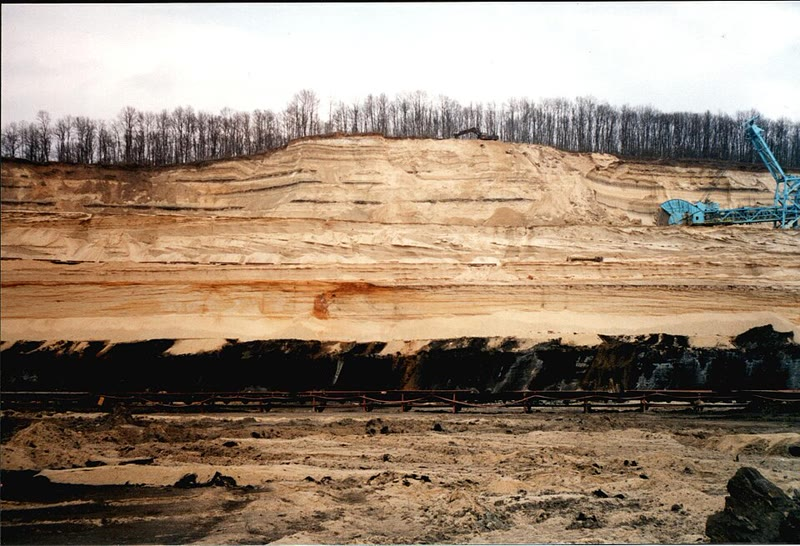
\includegraphics[height=4.0cm]{images/book2/g11-usgs-lignite-bed.jpg}};
\end{tikzpicture}

\medskip
\makebox[0.32\linewidth]{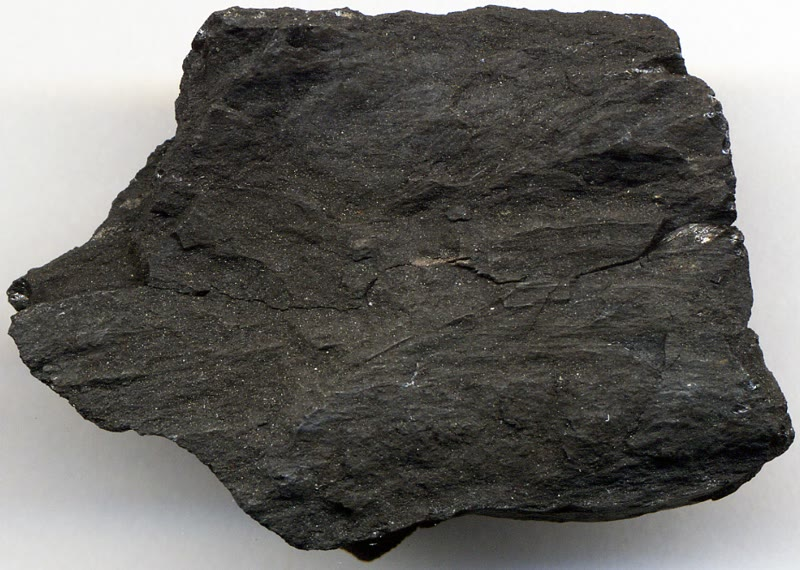
\includegraphics[height=3.2cm]{images/book2/g11-stjohn-lignite.jpg}}\hfill
\makebox[0.32\linewidth]{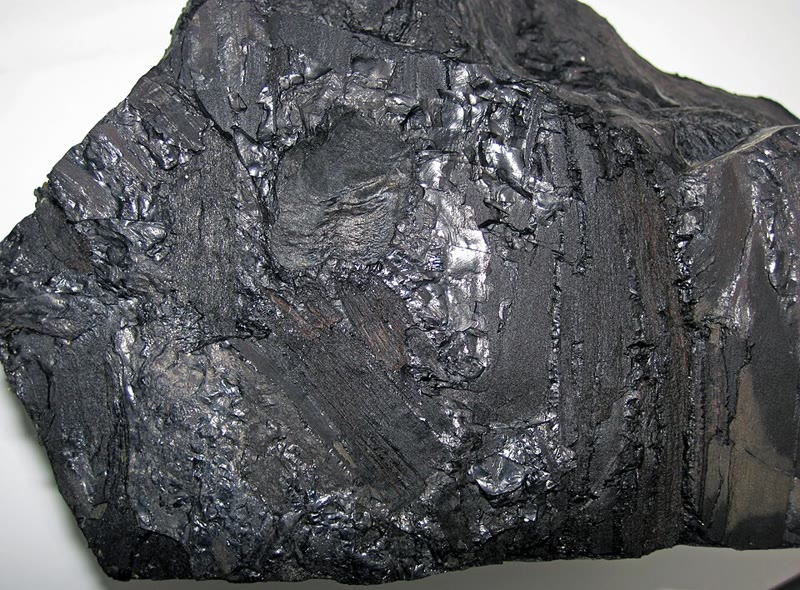
\includegraphics[height=3.2cm]{images/book2/g11-stjohn-bituminous.jpg}}\hfill
\makebox[0.32\linewidth]{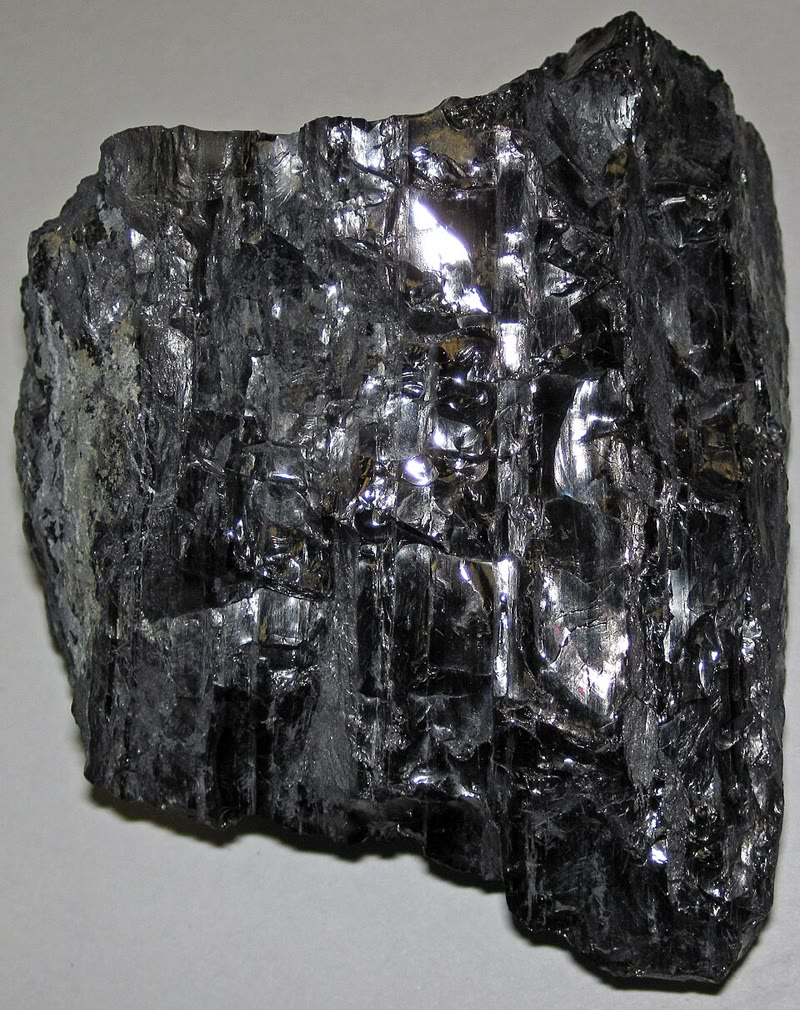
\includegraphics[height=3.2cm]{images/book2/g11-stjohn-anthracite.jpg}}

{\small Kiri atas: kandungan karbon \omterm{def:g11:fossil-fuel-geology:coal}{peringkat-peringkat} \omterm{def:g11:fossil-fuel-geology:coal}{batu bara}. Data: Badan
Informasi Energi Amerika Serikat. Kanan atas: selapis lignit, pita hitam di bawah
pasir yang pucat, yang tersingkap di sebuah tambang di Rumania; foto U.S.
Geological Survey (domain publik). Bawah, dari kiri: lignit, lebarnya sekitar
\qty{4.5}{cm}, cokelat kehitaman dan kusam; \omterm{def:g11:fossil-fuel-geology:coal}{batu bara} bituminus, dengan
pecahan-pecahan tumbuhan yang pipih; antrasit, hitam dan berkilap kaca. Foto
James St.~John (CC~BY~2.0).}
\end{omfigure}
% ledger: eia:coal-carbon, photo:g11-lignite-bed, photo:g11-coal-ranks

Gambut kehilangan sebagian besar volumenya di sepanjang jalan. Pada sebuah
lapisan \omterm{def:g11:fossil-fuel-geology:coal}{batu bara} di Utah bagian tengah, perbandingan antara gambut yang
terpotong oleh alur sungai purba dan \omterm{def:g11:fossil-fuel-geology:coal}{batu bara} yang hilang di sampingnya
memberikan rasio ketebalan sekitar $11{:}1$: setiap meter \omterm{def:g11:fossil-fuel-geology:coal}{batu bara} bituminus
itu dahulu adalah sekitar sebelas meter gambut.
% ledger: ryer80:peat-coal

\section{Latihan}

\begin{exercise}[$\star$]\label{exo:g11:fossil-fuel-geology:1}
Urutkan langkah-langkah yang mengarah dari plankton ke minyak bumi di dalam
\omterm{def:g11:fossil-fuel-geology:trap}{perangkap}: \omterm{def:g11:fossil-fuel-geology:migration}{migrasi}; \omterm{def:g11:fossil-fuel-geology:oil-window}{pematangan} dalam \omterm{def:g11:fossil-fuel-geology:oil-window}{jendela minyak}; penimbunan di bawah sedimen
yang lebih muda; plankton mati mengendap di dasar laut yang miskin oksigen;
minyak bumi berkumpul di bawah \omterm{def:g11:fossil-fuel-geology:reservoir}{batuan penutup}; bahan organik menjadi \omterm{def:g11:fossil-fuel-geology:source-rock}{kerogen} di
dalam lumpur.
\end{exercise}

\begin{exercise}[$\star$]\label{exo:g11:fossil-fuel-geology:2}
Untuk setiap batuan, katakan apakah batuan itu lebih mungkin menjadi \omterm{def:g11:fossil-fuel-geology:source-rock}{batuan
sumber}, \omterm{def:g11:fossil-fuel-geology:reservoir}{batuan reservoir}, atau \omterm{def:g11:fossil-fuel-geology:reservoir}{batuan penutup}: (1) serpih gelap yang kaya bahan
organik; (2) batu pasir yang terpilah baik dengan pori-pori yang saling
terhubung; (3) selapis garam; (4) batu lumpur tanpa bahan organik; (5) batu
kapur yang penuh rongga terbuka.
\end{exercise}

\begin{exercise}[$\star$]\label{exo:g11:fossil-fuel-geology:3}
Di sebuah cekungan, permukaannya bersuhu \qty{10}{\degreeCelsius} dan \omterm{def:g11:lithosphere-asthenosphere:geotherm}{gradien
geotermalnya} \qty{25}{\degreeCelsius/km}. Di antara kedalaman berapa \omterm{def:g11:fossil-fuel-geology:oil-window}{jendela
minyak} terletak? Berapa tebalnya?
\end{exercise}

\begin{exercise}[$\star$]\label{exo:g11:fossil-fuel-geology:4}
(1) Urutkan lignit, antrasit, \omterm{def:g11:fossil-fuel-geology:coal}{batu bara} bituminus, dan gambut menurut \omterm{def:g11:fossil-fuel-geology:coal}{peringkat}
yang naik. (2) Manakah yang kandungan karbonnya paling tinggi? (3) Manakah yang
terbentuk pada kedalaman dan suhu yang paling besar?
\end{exercise}

\begin{exercise}[$\star$]\label{exo:g11:fossil-fuel-geology:5}
(1) Di dalam \omterm{def:g11:fossil-fuel-geology:trap}{perangkap}, mengapa gas terletak di atas minyak bumi, dan minyak
bumi di atas air? (2) Mengapa batuan di atas reservoir harus kedap? Sebutkan
dua batuan yang menjadi \omterm{def:g11:fossil-fuel-geology:reservoir}{batuan penutup} yang baik.
\end{exercise}

\begin{exercise}[$\star\star$]\label{exo:g11:fossil-fuel-geology:6}
Dua cekungan mempunyai suhu permukaan yang sama, \qty{15}{\degreeCelsius}.
Cekungan A mempunyai gradien \qty{20}{\degreeCelsius/km}, cekungan B
\qty{40}{\degreeCelsius/km}. (1) Hitung kedalaman puncak dan dasar \omterm{def:g11:fossil-fuel-geology:oil-window}{jendela
minyak} di masing-masing cekungan. (2) Sebuah \omterm{def:g11:fossil-fuel-geology:source-rock}{batuan sumber} terletak pada
kedalaman \qty{2}{km} di kedua cekungan. Apa yang dihasilkannya di
masing-masing cekungan? (3) Di cekungan mana sebuah sumur harus menembus lebih
dalam untuk menemukan minyak bumi yang terbentuk di tempat?
\end{exercise}

\begin{exercise}[$\star\star$]\label{exo:g11:fossil-fuel-geology:7}
Ambil rasio $11{:}1$ yang diukur di Utah bagian tengah antara tebal gambut dan
tebal \omterm{def:g11:fossil-fuel-geology:coal}{batu bara} yang terbentuk darinya. (1) Berapa tebal gambut yang membentuk
lapisan \omterm{def:g11:fossil-fuel-geology:coal}{batu bara} setebal \qty{3}{m}? (2) Misalkan gambut itu menumpuk
\qty{1}{mm} setahun. Berapa lama waktu penumpukannya? (3) Mengapa rawa itu
pasti terus turun selama waktu itu?
\end{exercise}

\begin{exercise}[$\star\star$]\label{exo:g11:fossil-fuel-geology:8}
Gunakan diagram sejarah penimbunan Cekungan Merrow (permukaan
\qty{20}{\degreeCelsius}, gradien \qty{30}{\degreeCelsius/km}). \omterm{def:g11:fossil-fuel-geology:source-rock}{Batuan sumber}
berada pada kedalaman \qty{1.2}{km} 120 juta tahun yang lalu, \qty{2.3}{km} 95
juta tahun yang lalu, dan \qty{4.0}{km} 20 juta tahun yang lalu. (1) Hitung
suhunya pada setiap waktu itu. (2) Pada setiap waktu itu, apakah batuan itu
belum matang, berada dalam \omterm{def:g11:fossil-fuel-geology:oil-window}{jendela minyak}, atau dalam \omterm{def:g11:fossil-fuel-geology:oil-window}{jendela gas}?
\end{exercise}

\begin{exercise}[$\star\star$]\label{exo:g11:fossil-fuel-geology:9}
Bagian atas sebuah batu pasir reservoir membentuk lengkungan yang puncaknya
berada pada kedalaman \qty{2400}{m}; kontur tertutupnya yang terdalam berada
pada \qty{2580}{m}. Sebuah sumur di puncak menemukan gas sampai \qty{2450}{m},
lalu minyak bumi. (1) Berapa tinggi terbesar kolom yang dapat ditahan \omterm{def:g11:fossil-fuel-geology:trap}{perangkap}
itu? (2) Bila \omterm{def:g11:fossil-fuel-geology:trap}{perangkap} itu penuh, berapa tebal minyak buminya? (3) Minyak bumi
dan gas yang terus berdatangan setelah \omterm{def:g11:fossil-fuel-geology:trap}{perangkap} itu penuh: ke mana perginya?
\end{exercise}

\begin{exercise}[$\star\star$]\label{exo:g11:fossil-fuel-geology:10}
Bila tidak ada pengukuran \omterm{def:g11:fossil-fuel-geology:source-rock}{kerogen}, ahli geologi minyak bumi menganggap \omterm{def:g11:fossil-fuel-geology:source-rock}{batuan
sumber} yang terkubur di bawah lebih dari \qty{3}{km} batuan sebagai batuan yang
telah matang. Dengan permukaan bersuhu \qty{20}{\degreeCelsius}: (1) Gradien
berapa yang menempatkan \qty{3}{km} di puncak \omterm{def:g11:fossil-fuel-geology:oil-window}{jendela minyak}? di dasarnya?
(2) Dengan gradien 25 sampai \qty{34}{\degreeCelsius/km} yang diukur di lubang
bor, di mana letak \qty{3}{km}? Apakah aturan itu masuk akal?
\end{exercise}

\begin{exercise}[$\star\star$]\label{exo:g11:fossil-fuel-geology:11}
Tiga contoh \omterm{def:g11:fossil-fuel-geology:coal}{batu bara} mengandung \qty{30}{\percent}, \qty{70}{\percent}, dan
\qty{92}{\percent} karbon. (1) Sebutkan \omterm{def:g11:fossil-fuel-geology:coal}{peringkat} masing-masing. (2) Dengan
kedalaman dan suhu yang diberikan dalam pelajaran, manakah yang terkubur paling
dalam? (3) Lignit berpenampilan kusam dan cokelat kehitaman; bagaimana
penampilan antrasit?
\end{exercise}

\begin{exercise}[$\star\star\star$]\label{exo:g11:fossil-fuel-geology:12}
Antara 120 dan 95 juta tahun yang lalu, lumpur setebal \qty{1100}{m} menumpuk di
Cekungan Merrow. (1) Hitung laju penimbunannya dalam meter per sejuta tahun.
(2) Dengan gradien \qty{30}{\degreeCelsius/km}, berapa derajat \omterm{def:g11:fossil-fuel-geology:source-rock}{batuan sumber}
menghangat per sejuta tahun? (3) Seandainya laju ini terus berlangsung, berapa
lama \omterm{def:g11:fossil-fuel-geology:source-rock}{batuan sumber} memerlukan waktu untuk melintasi seluruh \omterm{def:g11:fossil-fuel-geology:oil-window}{jendela minyak}?
(4) Model itu memberikan sekitar 66 juta tahun. Mengapa lebih lama?
\end{exercise}

\begin{exercise}[$\star\star\star$]\label{exo:g11:fossil-fuel-geology:13}
Di Cekungan Merrow, \omterm{def:g11:fossil-fuel-geology:source-rock}{batuan sumber} berada dalam \omterm{def:g11:fossil-fuel-geology:oil-window}{jendela minyak} dari sekitar 117
sampai sekitar 51 juta tahun yang lalu, dan antiklin yang memerangkap minyak
bumi terbentuk 80 juta tahun yang lalu. (1) Anggaplah \omterm{def:g11:fossil-fuel-geology:source-rock}{batuan sumber} menghasilkan
minyak bumi dengan laju tetap selama berada di dalam jendela. Berapa bagian
minyak buminya yang terbentuk setelah \omterm{def:g11:fossil-fuel-geology:trap}{perangkap} itu ada? (2) Apa yang terjadi
pada sisanya? (3) Seandainya antiklin itu terbentuk 40 juta tahun yang lalu,
apa yang dapat ditahannya?
\end{exercise}

\begin{exercise}[$\star\star\star$]\label{exo:g11:fossil-fuel-geology:14}
Ambil sejarah penimbunan Cekungan Merrow (\cref{exo:g11:fossil-fuel-geology:8}:
\qty{0.4}{km} pada 150 juta tahun yang lalu, \qty{1.2}{km} pada 120, \qty{2.3}{km}
pada 95, \qty{3.0}{km} pada 66, dengan kedalaman yang bertambah secara tetap di
antaranya), tetapi untuk cekungan yang lebih panas: gradien
\qty{40}{\degreeCelsius/km}, permukaan \qty{20}{\degreeCelsius}. (1) Hitung
kedalaman puncak dan dasar \omterm{def:g11:fossil-fuel-geology:oil-window}{jendela minyak}. (2) Hitung umur ketika \omterm{def:g11:fossil-fuel-geology:source-rock}{batuan sumber}
memasuki dan meninggalkan jendela itu. (3) Antiklin itu tetap terbentuk 80
juta tahun yang lalu. Apakah antiklin itu akan menahan minyak bumi? Gas?
\end{exercise}

\begin{exercise}[$\star\star\star$]\label{exo:g11:fossil-fuel-geology:15}
Sebuah lapisan antrasit dari zaman Karbon kini tersingkap di permukaan. Zaman
Karbon berakhir sekitar 299 juta tahun yang lalu. (1) Dengan kedalaman yang
diberikan dalam pelajaran, seberapa dalam lapisan itu setidaknya pernah
terkubur? (2) Dengan permukaan bersuhu \qty{15}{\degreeCelsius} dan gradien
\qty{30}{\degreeCelsius/km}, suhu berapa yang dicapainya pada kedalaman itu?
Apakah suhu itu sesuai dengan suhu yang diberikan untuk antrasit? (3) Apa yang
telah terjadi pada batuan yang dahulu berada di atasnya? Berikan batas bawah
laju rata-ratanya, dalam milimeter per tahun, dengan menganggap semuanya terjadi
setelah zaman Karbon.
\end{exercise}

\section{Soal: Kapan Batuan Induk Menghasilkan Minyak Bumi?}

\begin{problem}[{Soal akhir pekan --- menentukan umur minyak bumi sebuah cekungan rekaan}]
\label{pb:g11:fossil-fuel-geology:1}
% values (oil_window.py): enter_oil_Ma 116.97, leave_oil_Ma 51.238, T_max 140, T_today 125,
% after_trap_frac 0.43757; ledger ics:base.Jurassic, ics:base.Cretaceous, earle:*, magoon00:tps
Sebuah sumur yang dibor menembus puncak sebuah antiklin di Cekungan Merrow,
sebuah cekungan rekaan, melintasi lapisan-lapisan di bawahnya. Setelah
ditentukan umurnya dari fosil-fosilnya, lapisan-lapisan itu merekam bagaimana
cekungan itu terisi. Dari yang tertua:
\begin{center}
\small
\begin{tabular}{|l|l|l|}
\hline
\textbf{selang (juta tahun yang lalu)} & \textbf{tebal} & \textbf{batuan} \\
\hline
165 sampai 150 & \qty{400}{m} & serpih hitam kaya bahan organik, lalu batu lumpur \\
150 sampai 120 & \qty{800}{m} & batu pasir berpori \\
120 sampai 95 & \qty{1100}{m} & batu lumpur \\
95 sampai 66 & \qty{700}{m} & kapur \\
66 sampai 35 & \qty{700}{m} & pasir dan lempung \\
35 sampai 20 & \qty{300}{m} & pasir \\
20 sampai kini & \qty{-500}{m} & pengangkatan: \qty{500}{m} teratas tererosi \\
\hline
\end{tabular}
\end{center}
Permukaannya bersuhu \qty{20}{\degreeCelsius} dan \omterm{def:g11:lithosphere-asthenosphere:geotherm}{gradien geotermalnya}
\qty{30}{\degreeCelsius/km}, keduanya dianggap tetap. Lapisan-lapisan itu
mempertahankan tebalnya setelah diendapkan (pemadatan diabaikan). Antiklin itu
terbentuk 80 juta tahun yang lalu. Ikutilah serpih hitam di dasar, yang
diendapkan 165 juta tahun yang lalu.

\medskip
\noindent\textbf{Bagian I --- Batuan.}
\begin{enumerate}
  \item Lapisan manakah yang menjadi \omterm{def:g11:fossil-fuel-geology:source-rock}{batuan sumber}, mana reservoir, dan mana
        \omterm{def:g11:fossil-fuel-geology:reservoir}{batuan penutup}?
  \item Apa yang membuat serpih hitam itu kaya bahan organik?
  \item Zaman Jura berlangsung dari sekitar \num{201.4} sampai \num{143.1} juta
        tahun yang lalu. Pada zaman apa \omterm{def:g11:fossil-fuel-geology:source-rock}{batuan sumber} itu diendapkan? Batu
        pasirnya?
  \item Apakah \omterm{def:g11:fossil-fuel-geology:source-rock}{kerogen} itu? Mengapa serpih hitam itu tidak menghasilkan minyak
        bumi di permukaan?
  \item Berapa tebal batuan yang kini berada di atas \omterm{def:g11:fossil-fuel-geology:source-rock}{batuan sumber}?
\end{enumerate}

\medskip
\noindent\textbf{Bagian II --- Penimbunan terhadap waktu.}
\begin{enumerate}[resume]
  \item Hitung kedalaman \omterm{def:g11:fossil-fuel-geology:source-rock}{batuan sumber} 150, 120, 95, 66, 35, dan 20 juta tahun
        yang lalu, dan kini.
  \item Hitung laju penimbunan, dalam meter per sejuta tahun, selama
        masing-masing dari enam selang pertama.
  \item Kapan \omterm{def:g11:fossil-fuel-geology:source-rock}{batuan sumber} berada paling dalam, dan seberapa dalam?
  \item Mengapa kedalamannya berkurang selama 20 juta tahun terakhir?
  \item Seberapa dalam dasar batu pasir itu kini?
\end{enumerate}

\medskip
\noindent\textbf{Bagian III --- Suhu terhadap waktu.}
\begin{enumerate}[resume]
  \item Hitung suhu \omterm{def:g11:fossil-fuel-geology:source-rock}{batuan sumber} pada setiap waktu dalam pertanyaan~6.
  \item Di antara kedalaman berapa \omterm{def:g11:fossil-fuel-geology:oil-window}{jendela minyak} terletak di cekungan ini?
  \item Di antara dua waktu manakah dalam pertanyaan~6 \omterm{def:g11:fossil-fuel-geology:source-rock}{batuan sumber} melewati
        \qty{60}{\degreeCelsius}?
  \item Dengan menganggap kedalamannya bertambah secara tetap dalam selang itu,
        hitung umur ketika batuan itu mencapai \qty{60}{\degreeCelsius}.
  \item Dengan cara yang sama, hitung kapan batuan itu mencapai
        \qty{120}{\degreeCelsius}.
\end{enumerate}

\medskip
\noindent\textbf{Bagian IV --- Masuk ke jendela, dan perangkapnya.}
\begin{enumerate}[resume]
  \item Berapa suhu tertinggi yang dicapainya? Apa yang dihasilkannya kini?
  \item Apa yang terjadi pada minyak bumi yang terbentuk sebelum antiklin itu
        ada?
  \item Dengan menganggap minyak bumi terbentuk dengan laju tetap selama \omterm{def:g11:fossil-fuel-geology:source-rock}{batuan
        sumber} berada di dalam jendela, berapa bagian minyak bumi yang terbentuk
        setelah antiklin itu ada?
  \item Fluida apa saja yang akan dijumpai sumur itu di puncak antiklin, dan
        dalam urutan apa dari atas?
  \item Simpulkan: kapan \omterm{def:g11:fossil-fuel-geology:source-rock}{batuan sumber} memasuki \omterm{def:g11:fossil-fuel-geology:oil-window}{jendela minyak}?
\end{enumerate}
\end{problem}
